\subsection{Optimizer comparison protocol}
\label{sec:optimizer-comparison}

We trained Model~B with Adam at $\alpha=10^{-3}$, plain stochastic gradient
descent (SGD) at $\alpha=10^{-2}$, and SGD at the same learning rate with
momentum $m=0.9$.  The model, split manifest, seed, data order, batch size and
augmentation were the same across runs.  Each run used seed 42, batch size
128, 30 epochs, zero weight decay, and a fixed learning rate without a
scheduler.  The sweep checks these shared settings before training.  The
saved Adam configuration uses \texttt{device: auto} and the SGD configurations
use \texttt{device: cuda}; all three profiles record a Tesla T4.

SGD updates the weights by
\begin{equation}
  w \leftarrow w-\alpha\frac{\partial L(w)}{\partial w},
\end{equation}
With momentum, the update is
\begin{equation}
  v \leftarrow mv-\alpha\frac{\partial L(w)}{\partial w},
  \qquad w \leftarrow w+v.
\end{equation}
Comparing $m=0$ and $m=0.9$ at the same SGD learning rate isolates the effect
of momentum.  Adam uses running first and second moments of the gradients
to scale each parameter's step.  We used its default coefficients,
$\beta_1=0.9$, $\beta_2=0.999$, and $\epsilon=10^{-8}$.

The learning rates $10^{-3}$ for Adam and $10^{-2}$ for SGD were starting
values for this comparison.  We did not run a learning-rate search for each
optimizer.  The results therefore apply to these configurations and this
training budget; each configuration was tested with one seed.

We selected Adam at $\alpha=10^{-3}$ for the custom-model runs because it
had the lowest validation loss (Table~\ref{tab:optimizer-comparison}).  It
also had the highest selected-checkpoint validation accuracy and test
accuracy among the three runs.  SGD with momentum reduced validation loss
faster than plain SGD over the 30 epochs.  For every run, the reported
metrics come from the lowest-validation-loss checkpoint.  Test accuracy
was used only for final evaluation.

\begin{table}[htbp]
  \centering
  \small
  \resizebox{\linewidth}{!}{\begin{tabular}{lrrrrrr}
\hline
Optimizer & LR & Momentum & Best val. loss & Best val. acc. (\%) & Test acc. (\%) & Epoch (s) \\
\hline
Adam & 0.001 & 0.0 & 0.427 & 84.42 & 83.75 & 11.61 \\
SGD & 0.01 & 0.0 & 1.996 & 23.14 & 23.48 & 11.12 \\
SGD + momentum & 0.01 & 0.9 & 0.471 & 83.56 & 82.86 & 11.02 \\
\hline
\end{tabular}
}
  \caption{Optimizer comparison for Model~B.  All runs use the same Tesla T4,
  split, seed, data order, batch size, augmentation, and 30-epoch budget.
  Validation accuracy is from the lowest-validation-loss checkpoint, not
  necessarily the maximum-accuracy epoch.  $m$ applies only to SGD; Adam uses
  its own moment coefficients.  Epoch time is the mean training-pass time,
  excluding validation.}
  \label{tab:optimizer-comparison}
\end{table}

\begin{figure}[H]
  \centering
  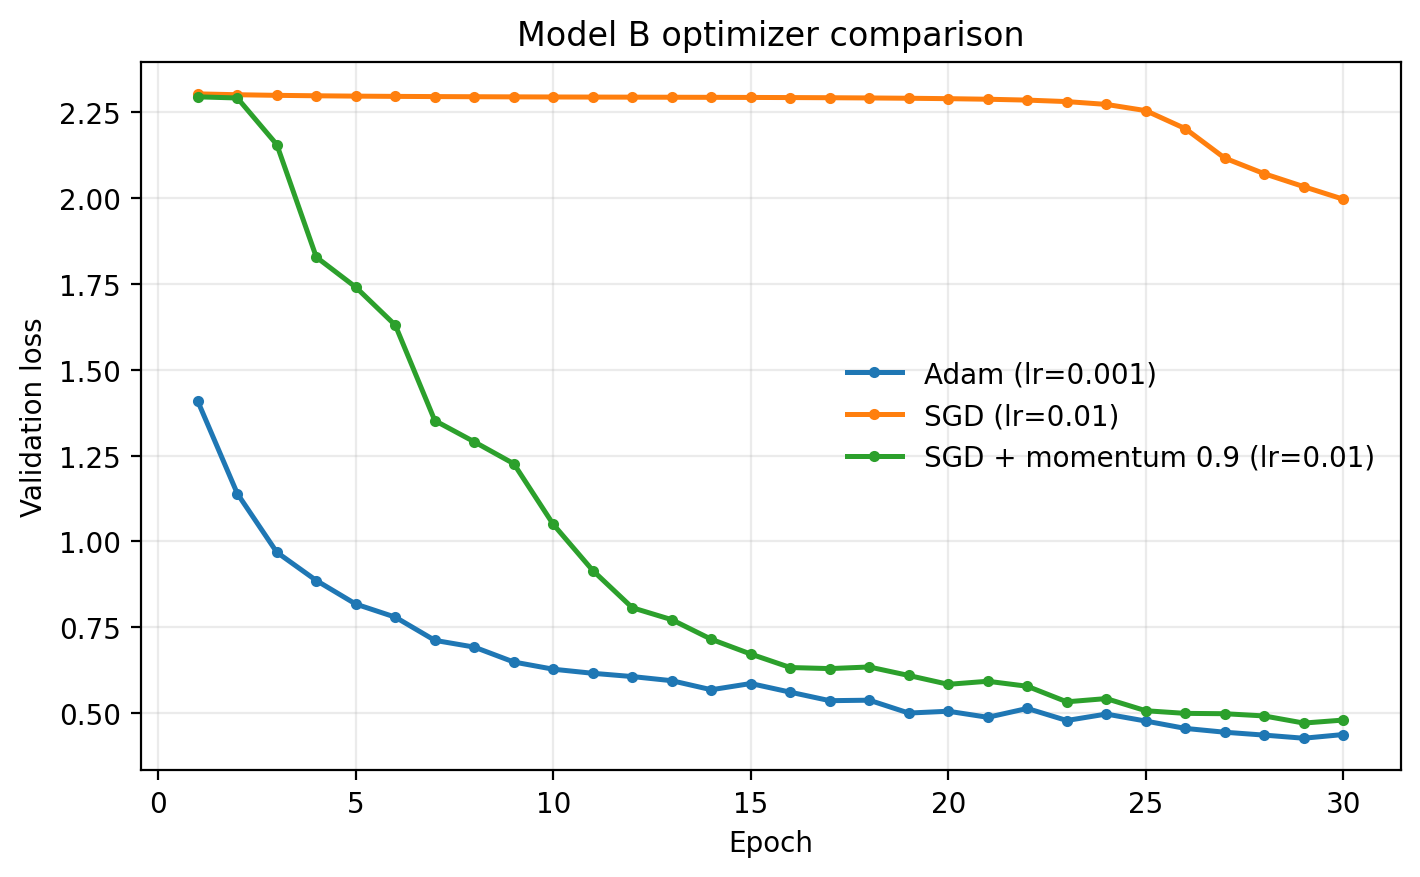
\includegraphics[width=0.86\linewidth]{figures/optimizer_comparison.png}
  \caption{Validation-loss comparison for Adam, plain SGD, and SGD with
  momentum on Model~B under an otherwise identical training budget.}
  \label{fig:optimizer-comparison}
\end{figure}

\subsection{Effect of the momentum coefficient}
\label{sec:momentum-ablation}

We compared SGD with $m\in\{0,0.5,0.9,0.99\}$ at the fixed learning
rate $\alpha=10^{-2}$.  The split, seed, data order, augmentation, batch size,
initialisation and 30-epoch budget were identical.  All four runs used an
NVIDIA GeForce RTX~3060 Laptop GPU.  Figure~\ref{fig:momentum-ablation}
uses the separate \texttt{momentum\_m000}, \texttt{momentum\_m050},
\texttt{momentum\_m090}, and \texttt{momentum\_m099} records.  Their epoch
times cannot be compared directly with the T4 runs in
Table~\ref{tab:optimizer-comparison}.

In the momentum update,
\begin{equation}
  v \leftarrow mv-\alpha\frac{\partial L(w)}{\partial w},
  \qquad w \leftarrow w+v,
  \label{eq:momentum-update}
\end{equation}
$m$ determines how much of the previous velocity is kept.  Gradients with a
consistent sign accumulate in $v$, increasing movement in that direction.
Across a narrow loss ravine, alternating gradient components cancel part of
the stored velocity, damping side-to-side motion.

With $m=0$, the update has no memory and validation loss stays high over the
epoch budget.  At $m=0.5$, loss falls sooner but is still high after 30 epochs.
At $m=0.9$, validation loss falls with small epoch-to-epoch fluctuations
and reaches the lowest value.  At $m=0.99$, loss falls fastest initially,
then fluctuates during later epochs and finishes above its selected minimum.
Keeping more past velocity could explain these fluctuations, but the saved
loss curves do not record gradient directions or establish overshooting.

We selected $m=0.9$ by validation loss.  The slightly higher test accuracy
at $m=0.99$ did not affect that choice.  This ranking is based on one run per
setting; its consistency across random seeds has not been measured.

\begin{figure}[H]
  \centering
  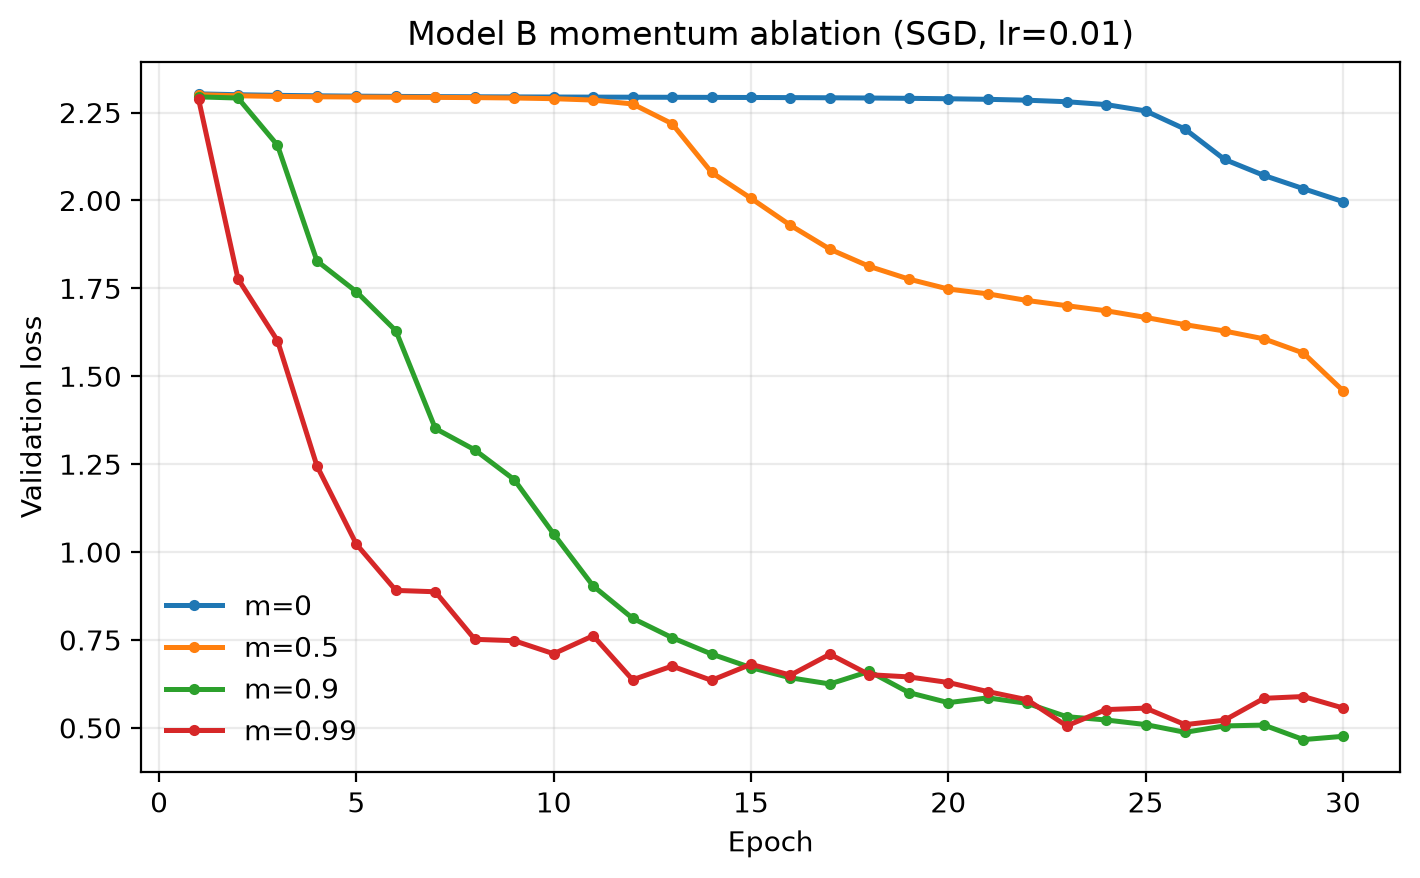
\includegraphics[width=0.86\linewidth]{figures/momentum_ablation.png}
  \caption{Validation-loss curves for Model~B with SGD at
  $\alpha=10^{-2}$.  Momentum is the only methodological variable across the
  four 30-epoch runs.}
  \label{fig:momentum-ablation}
\end{figure}
